\documentclass[12pt]{article}

\usepackage{a4wide}
\usepackage[utf8]{inputenc}
\usepackage[english]{babel}

\usepackage{amsmath}
\usepackage{biblatex}
\usepackage{courier}
\usepackage{csquotes}
\usepackage{enumerate}
\usepackage{graphicx}
\usepackage{listings}
\usepackage{svg}
\usepackage{color}

\definecolor{backcolour}{rgb}{0.95,0.95,0.92}

\lstdefinestyle{vcode}{
  backgroundcolor=\color{backcolour},
  basicstyle=\ttfamily\footnotesize,
  breaklines=true
}

\lstset{style=vcode}

\addbibresource{ref.bib}

\begin{document}

\title{Machine Learning Nanodegree: Capstone Project}
\author{Finbar Good}
\date{December 8, 2018}

\maketitle
   
\setlength{\parindent}{0cm}
\setlength{\parskip}{0.5\baselineskip}

\section{I. Definition}\label{i.-definition}

\emph{(approx. 1-2 pages)}

\subsection{Project Overview}\label{project-overview}
Since Google coined the term ``knowledge graph'', there has been an
increasing interest in the types of systems that fall under this broad
term\cite{ehrlinger2016towards}. Despite the interest - or perhaps
because of the lure of the name behind it - the term has been applied
widely and inconsistently. For the purposes of this proposal, we can
settle on this short definition: any store of facts represented as a
graph. And the sub-class of these graphs we are specifically interested
in are those that make use of the RDF standard.

RDF (Resource Description Framework) graphs \cite{w3RDF} represent facts
as a triple of IRIs or literal values. A triple consists of three parts:

\begin{itemize}
\item a subject: a thing or class, referred to using an IRI
\item a predicate: a property or relationship of the subject
\item an object: either the value subject's property, or the target of
  relationship
\end{itemize}

When the content of a graph is specified with RDF, the subjects and
objects form the nodes and the predicates form the edges. Because the
predicates are directed - going from subject to object - the graph is
directed.

\begin{figure}
  \centering
  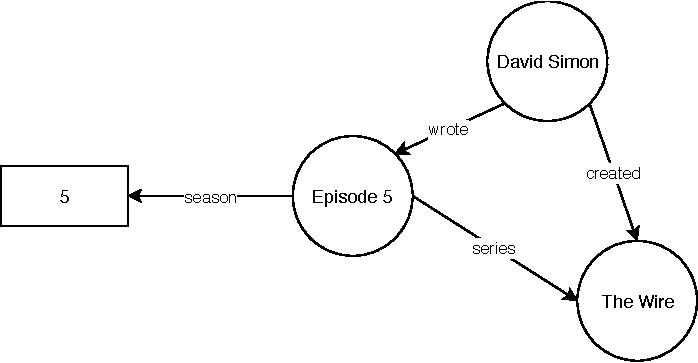
\includegraphics{images/rdf-the-wire.pdf}
  \caption{RDF example: some facts about The Wire}
\end{figure}

SPARQL is a query language designed for accessing RDF data, and was
elevated by the W3C to the recommended language for doing so
\cite{w3cSPARQL}. The following is an example of a very simple query in
SPARQL:

\begin{lstlisting}[language=SPARQL]
  SELECT ?creator
  WHERE { ?creator imbdo:created imdbr:the_wire }
\end{lstlisting}

In this example, we are looking for the entity (or entities) that
created another entity, imdbr:the\_wire. There are superficial
similarities with SQL, but they work in very distinct ways. What they
have in common is, from the point of view of a lay user, a steep
learning curve; only specialists tend to have the skills to create
queries in either language.

\subsection{Problem Statement}\label{problem-statement}
An area of research that has emerged in the past decade has been to
broaden the accessibility of knowledge graphs through parsing of natural
language queries (NLQ) to extract an answer from a knowledge graph (for
example \cite{Yahya:2012:NLQ:2390948.2390995}). Some of the more recent
efforts in the more general topic of question answering with a knowledge
base have looked at using neural networks to solve the problem (for
example \cite{liang2016neural}).

The challenge with accessing the data in knowledge graphs using RDF is
the query language, SPARQL. For many casual or non-technical users it is
an insurmountable barrier. To broaden the reach of such knowledge graphs
requires the automated translation of what casual users can produce,
natural language queries (NLQ), into something knowledge graphs can
parse, SPARQL.

This project aims to show that, at least in principal, a neural network
is a viable solution to automated translation of NLQs to SPARQL. Specifically:

\begin{enumerate}
  \item Download, merge, clean and split the LC-QuAD dataset (see \ref{data-exploration})
  \item Construct a word-oriented encoder-decoder neural network for training the translater
  \item Construct a SPARQL inference model that uses the trained encoder-decoder
  \item Train the encoder-decoder with the datasets
  \item Evaluate effectiveness of the inference model using the BLEU metric
  \item Repeat, altering hyper-parameters to investigate drivers of accuracy
\end{enumerate}

The models will be useful for considering the best approach to 
constructing a real, production-ready NLQ-to-SPARQL translater, supporting
search of a knowledge graph. Two key constraints are:
\begin{enumerate}
  \item Training datasets will, at least initially, be necessarily small
  \item The predicted SPARQL must be valid
\end{enumerate}

\subsection{Metrics}\label{metrics}

The BLEU score measures the degree of match between a generated sentence
and the reference sentence. This makes it useful to measure success of a
translation, in our case from natural language to SPARQL query. Values
range from 1 (perfect match) to 0 (perfect mismatch). Roughly, it is a
count of the number of distinct n-gram matches found in the reference
sentence, normalised by word count.

To use an example given in \cite{papineni2002bleu}, we have the
generated sentence:
  
\begin{lstlisting}[]
  It is a guide to action which ensures that the military always obeys the
  commands of the party
\end{lstlisting}

If we compare it to this reference sentence:

\begin{lstlisting}[]
  It is a guide to action that ensures that the military will forever heed
  Party commands
\end{lstlisting}

we see that 8 of the bigrams in the generated sentence are found in the
reference sentence. The bigram precision score is the number of matches
divided by the number of bigrams generated i.e.~8 / 17 = 0.47.

Shorter n-gram scores score precision, longer ones score fluency.

The actual calculation combines a precision measure with a penalty for 
the generated sentence being shorter than the reference sentence/s, the
brevity penalty. The brevity penalty is defined as:

\[ BP =
  \begin{cases}
    1               & \quad \text{if } c > r\\
    {\rm e}^{1-r/c} & \quad \text{if } c \leq r
  \end{cases}
\]

where c is the length of the candidate translation and r the reference
corpus length.

The BLEU score is then calculated as:

\[ BLEU = BP \cdot {\rm exp} \left( \sum_{n=1}^{N} w_n \log p_n \right) \]

where the weighted sum of n-gram precisions \(p_n\), up to \(N\), with weights \(w_n\).

I will use the BLEU metric to compare different training runs on the models.
As SPARQL queries are not ``fault tolerant'', we will need high scores for n
\textgreater{} 1.

\section{II. Analysis}\label{ii.-analysis}

\emph{(approx. 2-4 pages)}

\subsection{Data Exploration}\label{data-exploration}

In this section, you will be expected to analyze the data you are using
for the problem. This data can either be in the form of a dataset (or
datasets), input data (or input files), or even an environment. The type
of data should be thoroughly described and, if possible, have basic
statistics and information presented (such as discussion of input
features or defining characteristics about the input or environment).
Any abnormalities or interesting qualities about the data that may need
to be addressed have been identified (such as features that need to be
transformed or the possibility of outliers). Questions to ask yourself
when writing this section: - \emph{If a dataset is present for this
problem, have you thoroughly discussed certain features about the
dataset? Has a data sample been provided to the reader?} - \emph{If a
dataset is present for this problem, are statistics about the dataset
calculated and reported? Have any relevant results from this calculation
been discussed?} - \emph{If a dataset is \textbf{not} present for this
problem, has discussion been made about the input space or input data
for your problem?} - \emph{Are there any abnormalities or
characteristics about the input space or dataset that need to be
addressed? (categorical variables, missing values, outliers, etc.)}

\begin{center}\rule{0.5\linewidth}{\linethickness}\end{center}

The LC-QuAD dataset \cite{trivedi2017lc} was created
for the QALD (Question Answering over Linked Data) initiative
\cite{QALD}, a series of annual challenges to translate NLQ into SPARQL
(or the correct answer to the NLQ). The LC-QuAD dataset consists of 5000
questions and their corresponding SPARQL queries. The questions were
generated using the following workflow:

\begin{enumerate}
\def\labelenumi{\arabic{enumi}.}
\item
  Manually create query templates and a natural language equivalent
  template
\item
  Extract a list of entities
\item
  Manually create a whitelist of predicates
\item
  For each entity, extract subgraph centred on the entity from DBpedia,
  extending 2 hops away
\item
  Generate a query from each fact in these subgraphs, restricted to the
  predicate whitelist
\item
  The populated template is then mapped to the natural language
  equivalent
\item
  Humans review the final result, paraphrasing and/or correcting the
  results
\end{enumerate}

Here is an example entry from the dataset:

\begin{lstlisting}[]
  {
    "_id": "285", 
    "corrected_question": "In which state is the Channel district?", 
    "intermediary_question": "What is the <state> of Channel District ?", 
    "sparql_query": " SELECT DISTINCT ?uri WHERE { <http://dbpedia.org/resource/Channel_District> <http://dbpedia.org/ontology/state> ?uri } ", 
    "sparql_template_id": 2
  }
\end{lstlisting}

In this exercise, we are only interested in 2 fields:

\begin{itemize}
  \item corrected\_question: the natural language question
  \item sparql\_query: the target SPARQL query
\end{itemize}

\textbf{Query}
\begin{lstlisting}[language=SPARQL]
  SELECT DISTINCT ?url
  WHERE {
    { ?x dbp:league dbr:Turkish\_Handball\_Super\_League . }
    { ?x dbp:mascot ?uri }
  }
\end{lstlisting}

\textbf{Normalised Natural Question Template}
\begin{lstlisting}[]
What is the mascot of the handball team whose
league is Turkish Handball Super League?
\end{lstlisting}

\textbf{Corrected Question}
\begin{lstlisting}[]
What are the mascots of the teams participating in
the turkish handball super league?
\end{lstlisting}

\subsection{Exploratory Visualization}\label{exploratory-visualization}

In this section, you will need to provide some form of visualization
that summarizes or extracts a relevant characteristic or feature about
the data. The visualization should adequately support the data being
used. Discuss why this visualization was chosen and how it is relevant.
Questions to ask yourself when writing this section: - \emph{Have you
visualized a relevant characteristic or feature about the dataset or
input data?} - \emph{Is the visualization thoroughly analyzed and
discussed?} - \emph{If a plot is provided, are the axes, title, and
datum clearly defined?}

\begin{center}\rule{0.5\linewidth}{\linethickness}\end{center}

ideas:

\begin{itemize}
\item
  distribution of word frequencies
\item
  non-alpha chars
\item
  are there any ways to easily visualise word embedding distributions?
\end{itemize}

\subsection{Algorithms and Techniques}\label{algorithms-and-techniques}

In this section, you will need to discuss the algorithms and techniques
you intend to use for solving the problem. You should justify the use of
each one based on the characteristics of the problem and the problem
domain. Questions to ask yourself when writing this section: - \emph{Are
the algorithms you will use, including any default variables/parameters
in the project clearly defined?} - \emph{Are the techniques to be used
thoroughly discussed and justified?} - \emph{Is it made clear how the
input data or datasets will be handled by the algorithms and techniques
chosen?}

\begin{center}\rule{0.5\linewidth}{\linethickness}\end{center}

2 diagrams of LSTM, training and inference

\subsection{Benchmark}\label{benchmark}

In this section, you will need to provide a clearly defined benchmark
result or threshold for comparing across performances obtained by your
solution. The reasoning behind the benchmark (in the case where it is
not an established result) should be discussed. Questions to ask
yourself when writing this section: - \emph{Has some result or value
been provided that acts as a benchmark for measuring performance?} -
\emph{Is it clear how this result or value was obtained (whether by data
or by hypothesis)?}

\begin{center}\rule{0.5\linewidth}{\linethickness}\end{center}

I will be using the model described in \cite{soru2018neural} as the
benchmark. It defines the approach I will use, but uses a different
dataset. Both datasets were constructed from DBpedia, binding entities
found in DBPedia to question-query templates. The paper shows a number
of BLEU scores, one for each enhancement the team applied to their model
or dataset pre-processing.

\section{III. Methodology}\label{iii.-methodology}

\emph{(approx. 3-5 pages)}

\subsection{Data Preprocessing}\label{data-preprocessing}

In this section, all of your preprocessing steps will need to be clearly
documented, if any were necessary. From the previous section, any of the
abnormalities or characteristics that you identified about the dataset
will be addressed and corrected here. Questions to ask yourself when
writing this section: - \emph{If the algorithms chosen require
preprocessing steps like feature selection or feature transformations,
have they been properly documented?} - \emph{Based on the \textbf{Data
Exploration} section, if there were abnormalities or characteristics
that needed to be addressed, have they been properly corrected?} -
\emph{If no preprocessing is needed, has it been made clear why?}

\begin{center}\rule{0.5\linewidth}{\linethickness}\end{center}

\begin{itemize}
\item
  the source JSON format needs to be separated into the NLQ and SPARQL
  sets
\item
  punctuation needs to be removed
\item
  the SPARQL queries need to be encoded (it consists of special
  characters and urls as well as SPARQL keywords)
\end{itemize}

\subsection{Implementation}\label{implementation}

In this section, the process for which metrics, algorithms, and
techniques that you implemented for the given data will need to be
clearly documented. It should be abundantly clear how the implementation
was carried out, and discussion should be made regarding any
complications that occurred during this process. Questions to ask
yourself when writing this section: - \emph{Is it made clear how the
algorithms and techniques were implemented with the given datasets or
input data?} - \emph{Were there any complications with the original
metrics or techniques that required changing prior to acquiring a
solution?} - \emph{Was there any part of the coding process (e.g.,
writing complicated functions) that should be documented?}

\begin{center}\rule{0.5\linewidth}{\linethickness}\end{center}

For this proposed project I will be taking the same approach as
described in \cite{soru2018neural}, which is to use neural machine
translation to predicate SPARQL from NLQ.

\subsection{Refinement}\label{refinement}

In this section, you will need to discuss the process of improvement you
made upon the algorithms and techniques you used in your implementation.
For example, adjusting parameters for certain models to acquire improved
solutions would fall under the refinement category. Your initial and
final solutions should be reported, as well as any significant
intermediate results as necessary. Questions to ask yourself when
writing this section: - \emph{Has an initial solution been found and
clearly reported?} - \emph{Is the process of improvement clearly
documented, such as what techniques were used?} - \emph{Are intermediate
and final solutions clearly reported as the process is improved?}

\begin{center}\rule{0.5\linewidth}{\linethickness}\end{center}

\section{IV. Results}\label{iv.-results}

\emph{(approx. 2-3 pages)}

\subsection{Model Evaluation and Validation}\label{model-evaluation-and-validation}

In this section, the final model and any supporting qualities should be
evaluated in detail. It should be clear how the final model was derived
and why this model was chosen. In addition, some type of analysis should
be used to validate the robustness of this model and its solution, such
as manipulating the input data or environment to see how the model's
solution is affected (this is called sensitivity analysis). Questions to
ask yourself when writing this section: - \emph{Is the final model
reasonable and aligning with solution expectations? Are the final
parameters of the model appropriate?} - \emph{Has the final model been
tested with various inputs to evaluate whether the model generalizes
well to unseen data?} - \emph{Is the model robust enough for the
problem? Do small perturbations (changes) in training data or the input
space greatly affect the results?} - \emph{Can results found from the
model be trusted?}

\begin{center}\rule{0.5\linewidth}{\linethickness}\end{center}

\subsection{Justification}\label{justification}

In this section, your model's final solution and its results should be
compared to the benchmark you established earlier in the project using
some type of statistical analysis. You should also justify whether these
results and the solution are significant enough to have solved the
problem posed in the project. Questions to ask yourself when writing
this section: - \emph{Are the final results found stronger than the
benchmark result reported earlier?} - \emph{Have you thoroughly analyzed
and discussed the final solution?} - \emph{Is the final solution
significant enough to have solved the problem?}

\begin{center}\rule{0.5\linewidth}{\linethickness}\end{center}

\section{V. Conclusion}\label{v.-conclusion}

\emph{(approx. 1-2 pages)}

\subsection{Free-Form Visualization}\label{free-form-visualization}

In this section, you will need to provide some form of visualization
that emphasizes an important quality about the project. It is much more
free-form, but should reasonably support a significant result or
characteristic about the problem that you want to discuss. Questions to
ask yourself when writing this section: - \emph{Have you visualized a
relevant or important quality about the problem, dataset, input data, or
results?} - \emph{Is the visualization thoroughly analyzed and
discussed?} - \emph{If a plot is provided, are the axes, title, and
datum clearly defined?}

\begin{center}\rule{0.5\linewidth}{\linethickness}\end{center}

\subsection{Reflection}\label{reflection}

In this section, you will summarize the entire end-to-end problem
solution and discuss one or two particular aspects of the project you
found interesting or difficult. You are expected to reflect on the
project as a whole to show that you have a firm understanding of the
entire process employed in your work. Questions to ask yourself when
writing this section: - \emph{Have you thoroughly summarized the entire
process you used for this project?} - \emph{Were there any interesting
aspects of the project?} - \emph{Were there any difficult aspects of the
project?} - \emph{Does the final model and solution fit your
expectations for the problem, and should it be used in a general setting
to solve these types of problems?}

\begin{center}\rule{0.5\linewidth}{\linethickness}\end{center}

\subsection{Improvement}\label{improvement}

In this section, you will need to provide discussion as to how one
aspect of the implementation you designed could be improved. As an
example, consider ways your implementation can be made more general, and
what would need to be modified. You do not need to make this
improvement, but the potential solutions resulting from these changes
are considered and compared/contrasted to your current solution.
Questions to ask yourself when writing this section: - \emph{Are there
further improvements that could be made on the algorithms or techniques
you used in this project?} - \emph{Were there algorithms or techniques
you researched that you did not know how to implement, but would
consider using if you knew how?} - \emph{If you used your final solution
as the new benchmark, do you think an even better solution exists?}

\begin{center}\rule{0.5\linewidth}{\linethickness}\end{center}

\textbf{Before submitting, ask yourself. . .}

\begin{itemize}
\item
  Does the project report you've written follow a well-organized
  structure similar to that of the project template?
\item
  Is each section (particularly \textbf{Analysis} and
  \textbf{Methodology}) written in a clear, concise and specific
  fashion? Are there any ambiguous terms or phrases that need
  clarification?
\item
  Would the intended audience of your project be able to understand your
  analysis, methods, and results?
\item
  Have you properly proof-read your project report to assure there are
  minimal grammatical and spelling mistakes?
\item
  Are all the resources used for this project correctly cited and
  referenced?
\item
  Is the code that implements your solution easily readable and properly
  commented?
\item
  Does the code execute without error and produce results similar to
  those reported?
\end{itemize}

\printbibliography
   
\end{document}
